\documentclass[10pt,a4paper]{article}
\usepackage[utf8]{inputenc}
\usepackage{amsthm, amsmath, mathtools, amssymb}
\usepackage[left=2cm,right=2cm,top=2cm,bottom=2cm]{geometry}
\usepackage[colorlinks,linkcolor=blue,citecolor=blue,urlcolor=blue]{hyperref}
\usepackage[catalan]{babel}
\usepackage{titlesec}
\usepackage{enumitem}
\usepackage{physics}
\usepackage{fancyhdr}
\usepackage{subcaption}

\newcommand{\NN}{\ensuremath{\mathbb{N}}} % set of natural numbers
\newcommand{\ZZ}{\ensuremath{\mathbb{Z}}} % set of integers
\newcommand{\QQ}{\ensuremath{\mathbb{Q}}} % set of rationals
\newcommand{\RR}{\ensuremath{\mathbb{R}}} % set of real numbers
\newcommand{\CC}{\ensuremath{\mathbb{C}}} % set of complex numbers
\newcommand{\KK}{\ensuremath{\mathbb{K}}} % a general field

\newcommand{\vf}[1]{\boldsymbol{\mathrm{#1}}} % math style for vectors and matrices and vector-values functions (previously it was \*vb{#1} but this does not apply to greek letters)
\newcommand{\ii}{\mathrm{i}} % imaginary unit
\renewcommand{\O}{\mathrm{O}} % big O-notation

\newtheorem{theorem}{Teorema}
\newtheorem{exercici}{Exercice}
\newtheorem{prop}{Proposició}
\theoremstyle{definition}
\newtheorem{definition}{Definició}
\theoremstyle{remark}
\newtheorem*{res}{Resolution}
\DeclareDocumentCommand\derivative{ s o m g d() }{ 
  % Total derivative
  % s: star for \flatfrac flat derivative
  % o: optional n for nth derivative
  % m: mandatory (x in df/dx)
  % g: optional (f in df/dx)
  % d: long-form d/dx(...)
    \IfBooleanTF{#1}
    {\let\fractype\flatfrac}
    {\let\fractype\frac}
    \IfNoValueTF{#4}
    {
        \IfNoValueTF{#5}
        {\fractype{\diffd \IfNoValueTF{#2}{}{^{#2}}}{\diffd #3\IfNoValueTF{#2}{}{^{#2}}}}
        {\fractype{\diffd \IfNoValueTF{#2}{}{^{#2}}}{\diffd #3\IfNoValueTF{#2}{}{^{#2}}} \argopen(#5\argclose)}
    }
    {\fractype{\diffd \IfNoValueTF{#2}{}{^{#2}} #3}{\diffd #4\IfNoValueTF{#2}{}{^{#2}}}\IfValueT{#5}{(#5)}}
} % differential operator
\DeclareDocumentCommand\partialderivative{ s o m g d() }{ 
  % Total derivative
  % s: star for \flatfrac flat derivative
  % o: optional n for nth derivative
  % m: mandatory (x in df/dx)
  % g: optional (f in df/dx)
  % d: long-form d/dx(...)
  \IfBooleanTF{#1}
    {\let\fractype\flatfrac}
    {\let\fractype\frac}
    \IfNoValueTF{#4}{
      \IfNoValueTF{#5}
      {\fractype{\partial \IfNoValueTF{#2}{}{^{#2}}}{\partial #3\IfNoValueTF{#2}{}{^{#2}}}}
      {\fractype{\partial \IfNoValueTF{#2}{}{^{#2}}}{\partial #3\IfNoValueTF{#2}{}{^{#2}}} \argopen(#5\argclose)}
    }
    {\fractype{\partial \IfNoValueTF{#2}{}{^{#2}} #3}{\partial #4\IfNoValueTF{#2}{}{^{#2}}}\IfValueT{#5}{(#5)}}
} % partial differential operator

\titleformat{\section}
  {\normalfont\fontsize{11}{15}\bfseries}{\thesection}{1em}{}

% \renewcommand{\theenumi}{\textbf{\arabic{enumi}}}
\renewcommand{\theenumi}{\alph{enumi}}
\renewcommand{\theenumiii}{\roman{enumiii}}
\renewcommand{\exp}[1]{\mathrm{e}^{#1}} % exponential function
\DeclareMathOperator*{\im}{Im}

\title{\bfseries\Large Octave problems}

\author{Víctor Ballester Ribó\\NIU: 1570866}
\date{\parbox{\linewidth}{\centering
  Integració numèrica d'equacions en derivades parcials\endgraf
  Grau en Matemàtiques\endgraf
  Universitat Autònoma de Barcelona\endgraf
  Febrer de 2023}}
  \pagestyle{fancy}
  \fancyhf{}
  \fancyhfoffset[L]{1cm}
  \fancyhfoffset[R]{1cm}
  \rhead{NIU: 1570866}
  \lhead{Víctor Ballester}
  \cfoot{\thepage}
  %\setlength{\headheight}{13.6pt}

\setlength{\parindent}{0pt}
\begin{document}
\selectlanguage{catalan}
\maketitle
\begin{exercici}
  For values of $x\in[-1,3]$ and $t\in [0,2.4]$, compare the following numerical schemes for the one-dimensional wave equation
  $$
    u_t+u_x=0
  $$
  with initial condition
  $$
    u(0,x)=\begin{cases}
      {\cos(\pi x)}^2 & \abs{x}\leq \frac{1}{2} \\
      0               & \text{en cas otherwise}
    \end{cases}
  $$
  and boundary condition $u(t,-1)=0$. Use spatial time steps of $h=1/10$, $h=1/20$, and $h=1/40$.
  \begin{enumerate}
    \item Forward-time, backward-space (FTBS) with $\lambda =0.8$.
          \item\label{ex1:b} Forward-time, centered-space (FTCS) with $\lambda =0.8$.
          \item\label{ex1:c} Lax-Friedrichs (LF) with $\lambda =0.8$ and $\lambda =1.6$.
          \item\label{ex1:d} Leapfrog (L) with $\lambda =0.8$ and using the forward-time, centered-space scheme for the first step.
  \end{enumerate}
  For schemes \ref{ex1:b}, \ref{ex1:c}, and \ref{ex1:d}, use the numerical boundary condition $v_M^{n+1}=v_{M-1}^{n+1}$.
\end{exercici}
\begin{res}
  In the next table we expose the error in $L^\infty$ norm of all the experiments that we have done.
  \begin{table}[ht]
    \centering
    \begin{tabular}{l|c|c|c}
      Scheme               & $h=1/10$  & $h=1/20$    & $h=1/40$          \\
      \hline\hline
      FTBS ($\lambda=0.8$) & 0.309408  & 0.188814    & 0.105457          \\
      FTCS ($\lambda=0.8$) & 30.065494 & 4532.489959 & 2117202272.413460 \\
      LF ($\lambda=0.8$)   & 0.475755  & 0.331514    & 0.206424          \\
      LF ($\lambda=1.6$)   & 37.449901 & 3672.928504 & 771466658.304601  \\
      L ($\lambda=0.8$)    & 0.179728  & 0.076990    & 0.055387
    \end{tabular}
    \caption{Error in $L^\infty$ norm for the different schemes.}
  \end{table}
  From here we can conclude that the useful schemes are the FTBS with $\lambda=0.8$, the Lax-Friedrichs with $\lambda=0.8$ and the Leapfrog with $\lambda=0.8$. And the other ones are useless as the error seams to approach to infinity as we decrease the step size $h$. The next figures shows the solutions of the three convergent methods with the three spatial steps mentioned above.
  \begin{figure}[ht]
    \centering
    \begin{subfigure}{0.49\textwidth}
      \centering
      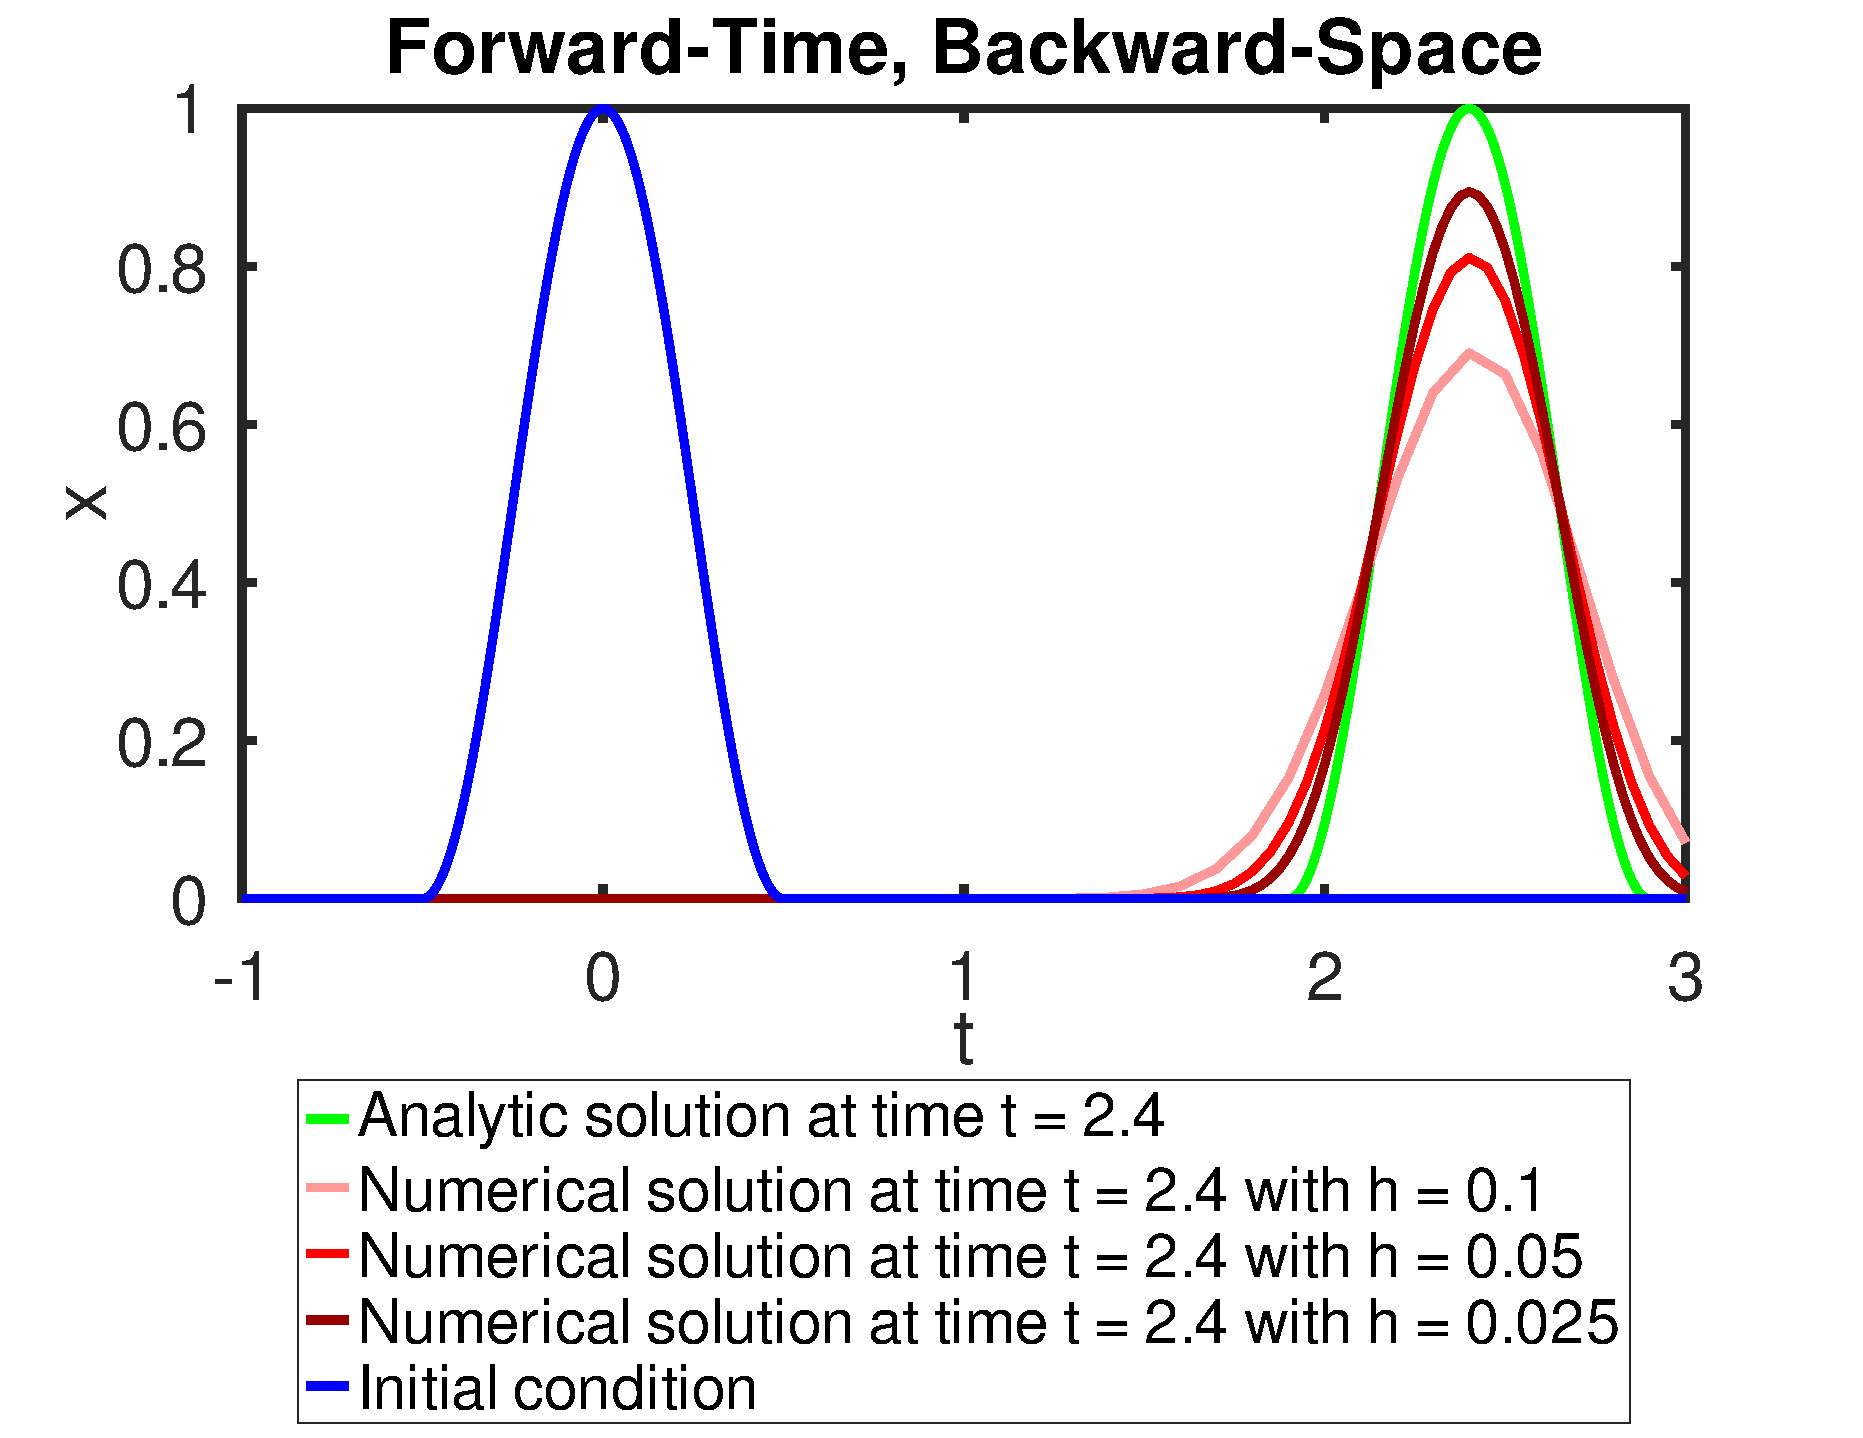
\includegraphics[width=\textwidth]{Images/ftbs.pdf}
      \caption{FTBS with $\lambda=0.8$.}
    \end{subfigure}\hfill
    \begin{subfigure}{0.49\textwidth}
      \centering
      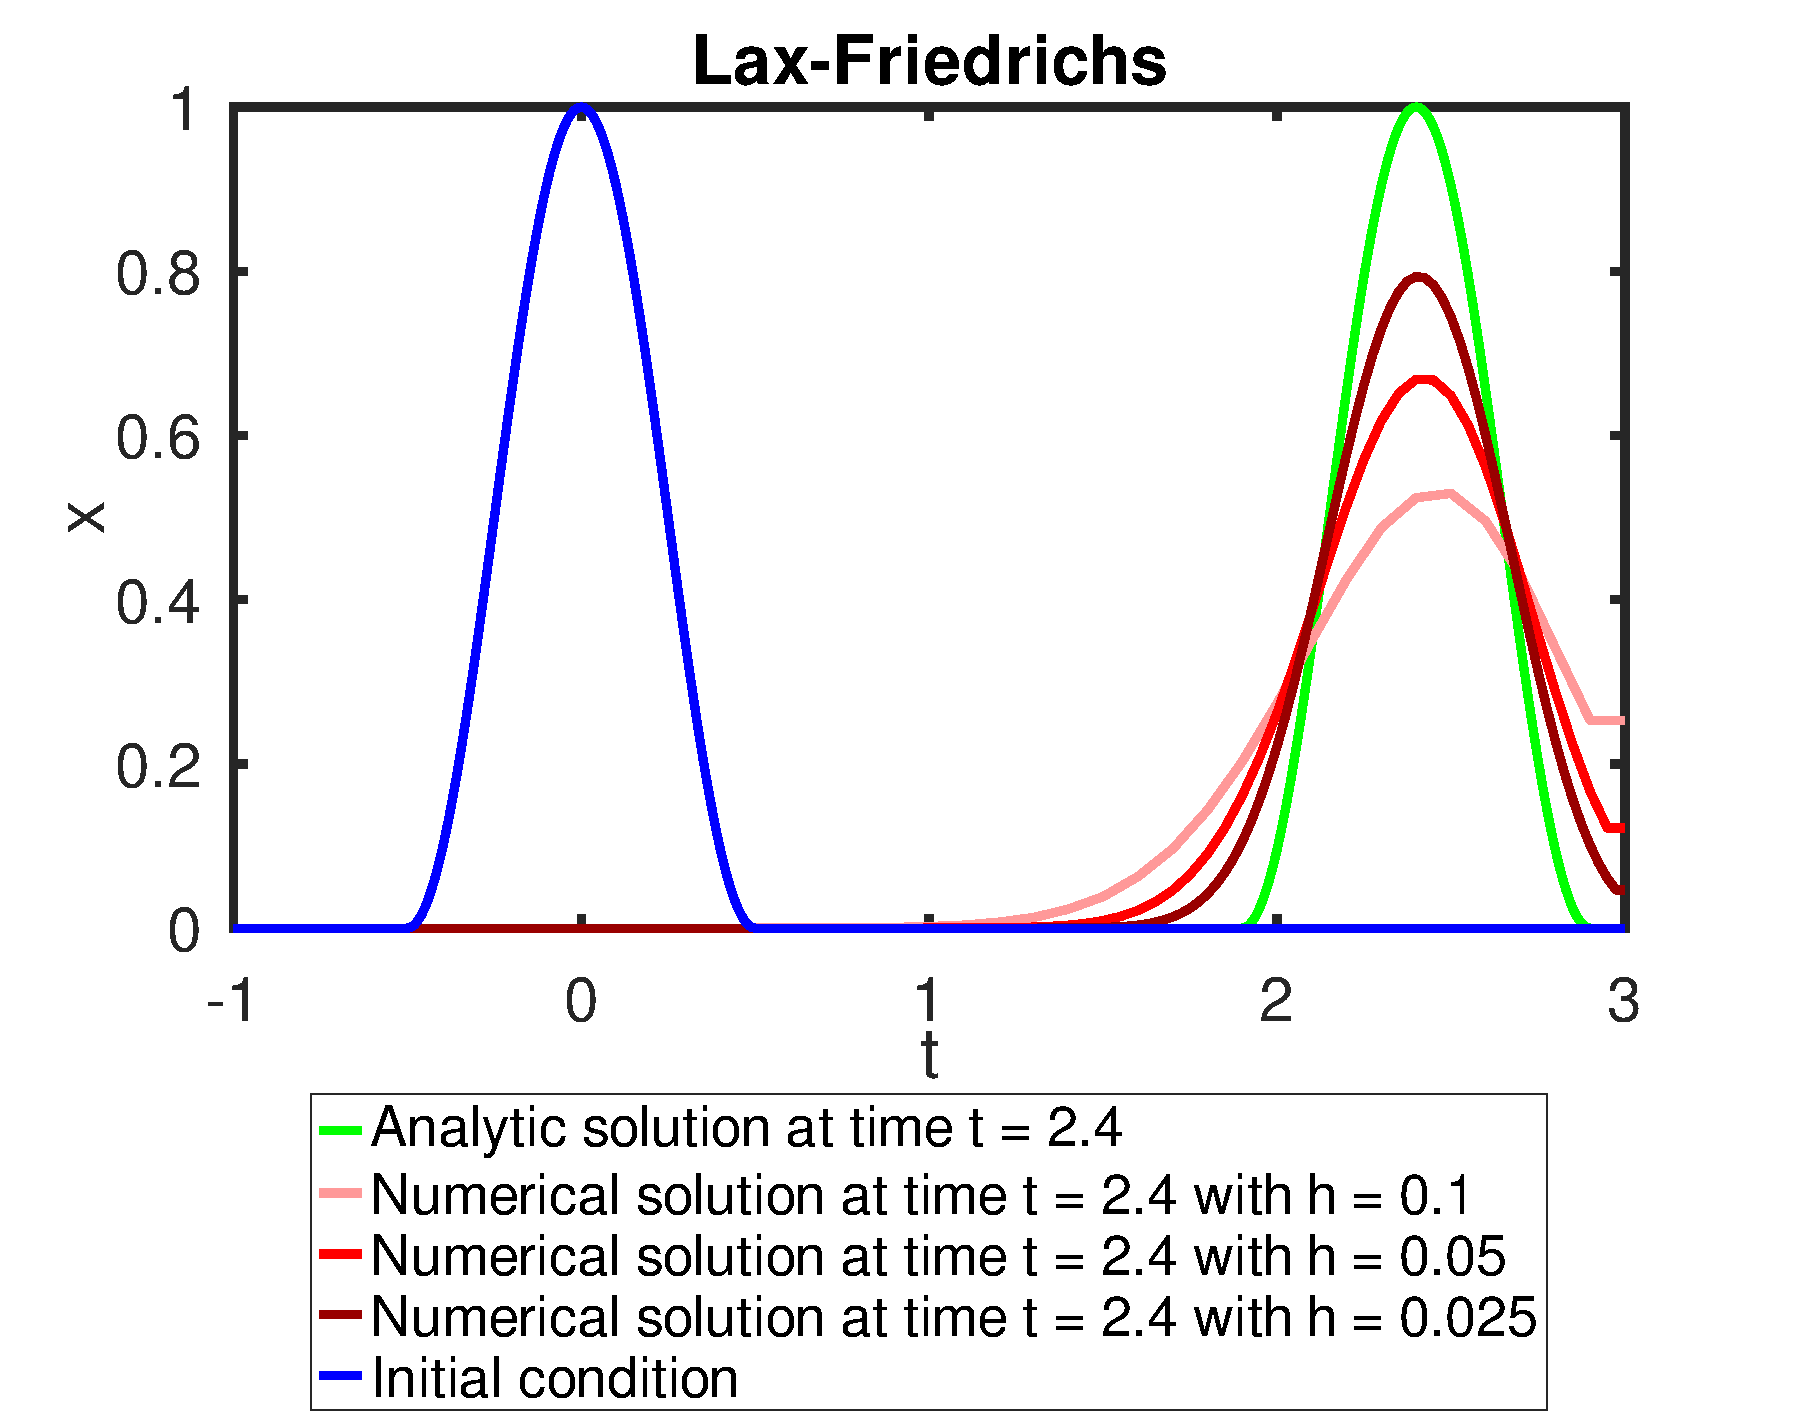
\includegraphics[width=\textwidth]{Images/lf.pdf}
      \caption{Lax-Friedrichs with $\lambda=0.8$.}
    \end{subfigure}\hfill
    \begin{subfigure}{0.49\textwidth}
      \centering
      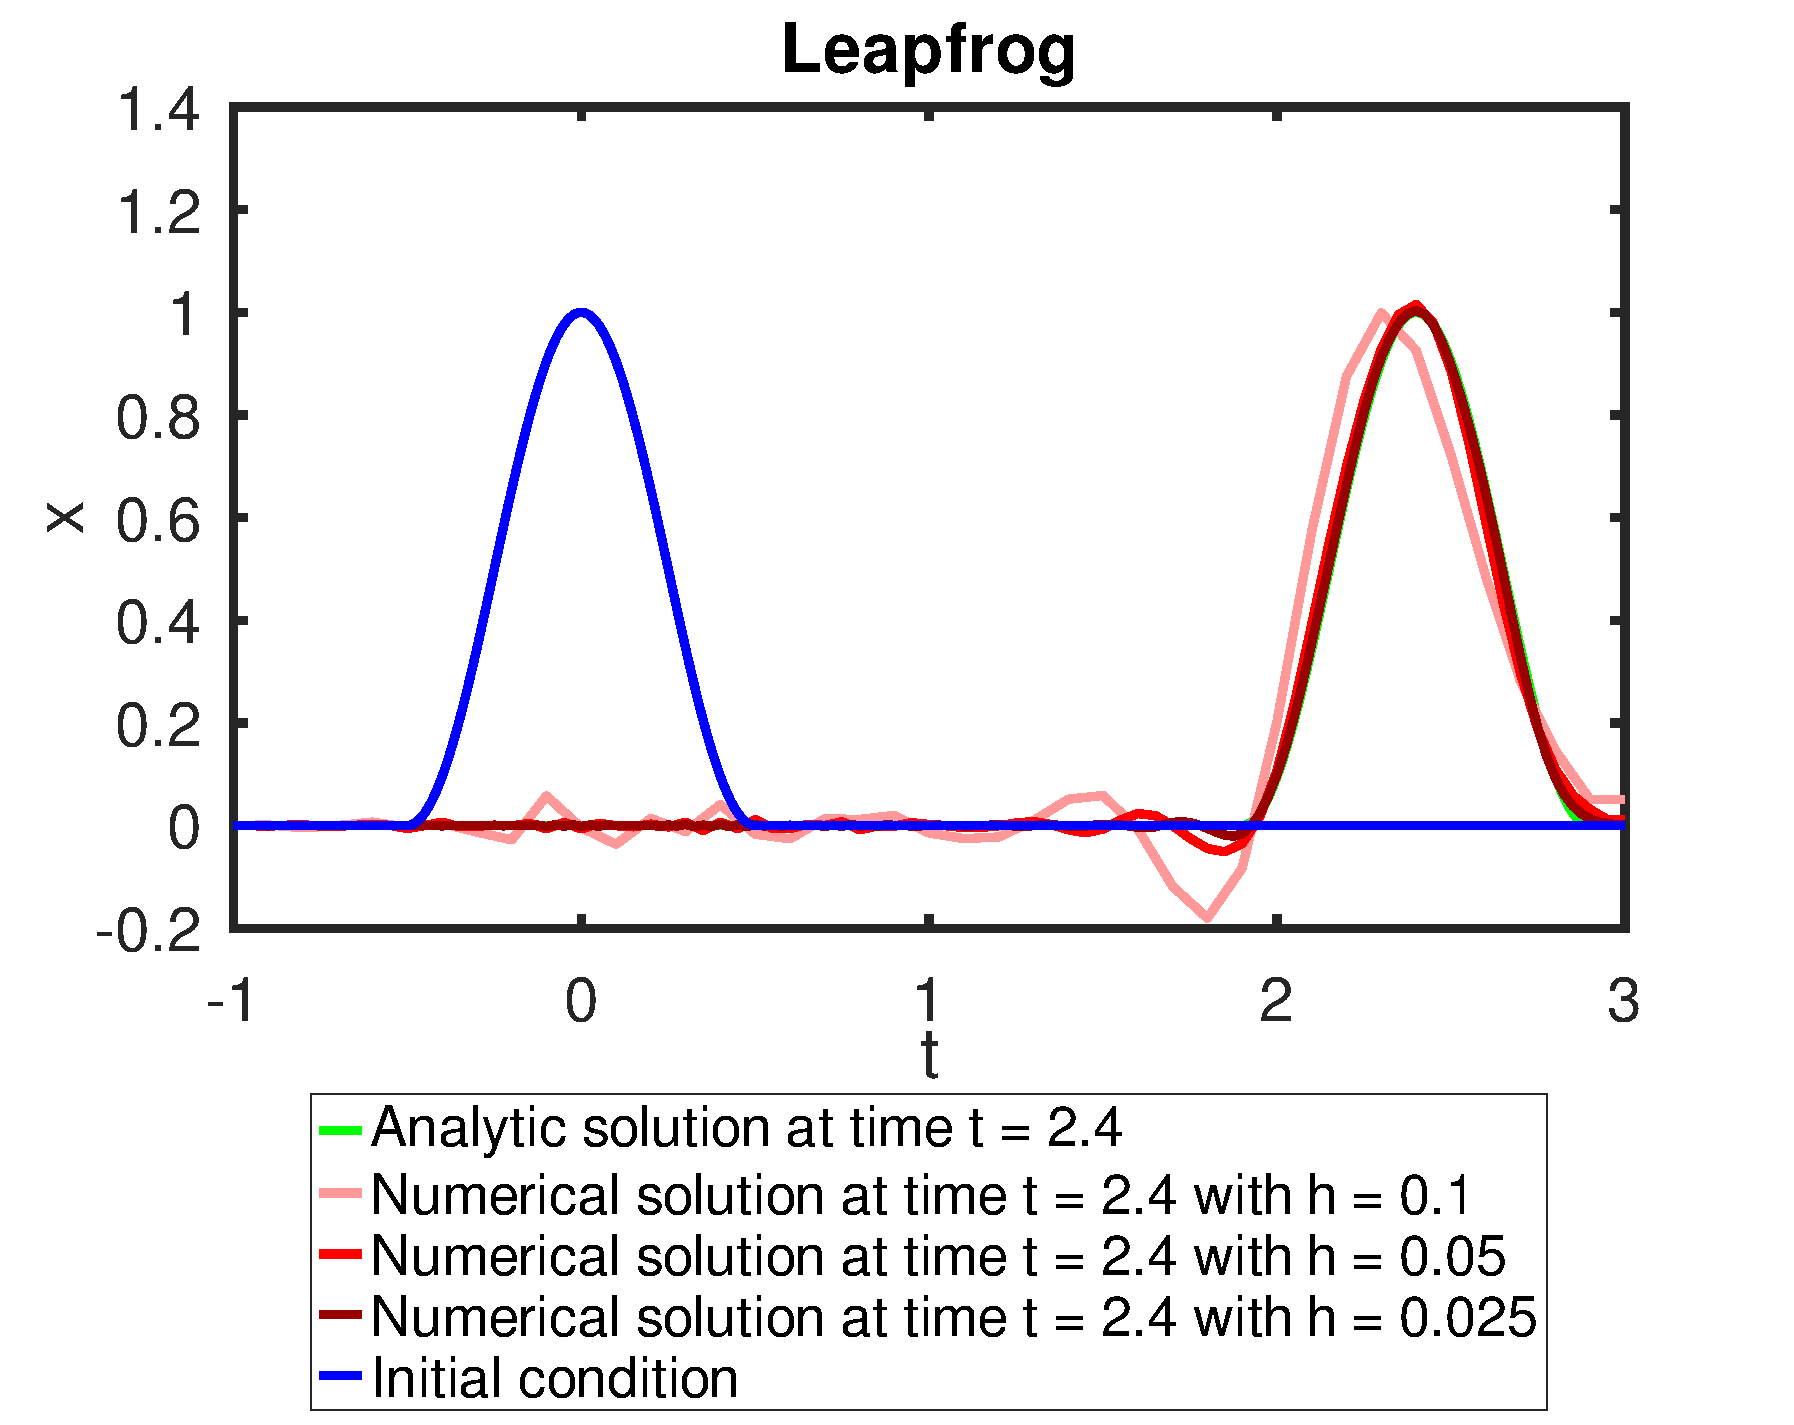
\includegraphics[width=\textwidth]{Images/l.pdf}
      \caption{Leapfrog with $\lambda=0.8$.}
    \end{subfigure}
    \caption{Plot of the analytical and numerical solutions of the convergent schemes}
  \end{figure}
\end{res}
\begin{exercici}
  Solve $u_t+u_x=0$, $x\in[-1,1]$, $t\in[0,2.1]$, with initial condition $u(0,x)=\sin(2\pi x)$ and periodicity $u(t,-1)=u(t,1)$. Use the following schemes:
  \begin{enumerate}
    \item Forward-time, backward-space (FTBS) with $\lambda =0.8$.
    \item Lax-Wendroff (LW) with $\lambda =0.8$.
  \end{enumerate}
  Demonstrate the first-order accuracy of the FTBS scheme and the second-order accuracy of the LW scheme using time steps of $h=1/10$, $h=1/20$, $h=1/40$ and $h=1/80$. Do it in both the norm $L^2$ and the norm $L^\infty$.
\end{exercici}
\begin{res}
  The next table summarizes all the experiments that we have done.
  \begin{table}[ht]
    \centering
    \begin{tabular}{|c|c|c|c|c||c|c|c|c|}
      \hline
             & \multicolumn{4}{c||}{FTBS} & \multicolumn{4}{c|}{LW}                                                                                                                 \\
      \cline{2-9}
             & \multicolumn{2}{c|}{$L^2$} & \multicolumn{2}{c||}{$L^\infty$} & \multicolumn{2}{c|}{$L^2$} & \multicolumn{2}{c|}{$L^\infty$}                                         \\
      \cline{2-9}
      $h$    & Error                      & Rate                             & Error                      & Rate                            & Error    & Rate   & Error    & Rate   \\
      \hline\hline
      $1/10$ & 0.379872                   & -                                & 0.371158                   & -                               & 0.169042 & -      & 0.166403 & -      \\
      $1/20$ & 0.211259                   & 1.7981                           & 0.210930                   & 1.7596                          & 0.044196 & 3.8248 & 0.043954 & 3.7858 \\
      $1/40$ & 0.111737                   & 1.8907                           & 0.111688                   & 1.8886                          & 0.011139 & 3.9677 & 0.011121 & 3.9523 \\
      $1/80$ & 0.057504                   & 1.9431                           & 0.057498                   & 1.9425                          & 0.002789 & 3.9939 & 0.002788 & 3.9889 \\
      \hline
    \end{tabular}
    \caption{Error in $L^\infty$ norm for the different schemes.}
  \end{table}
  \begin{figure}[ht]
    \centering
    \begin{subfigure}{0.49\textwidth}
      \centering
      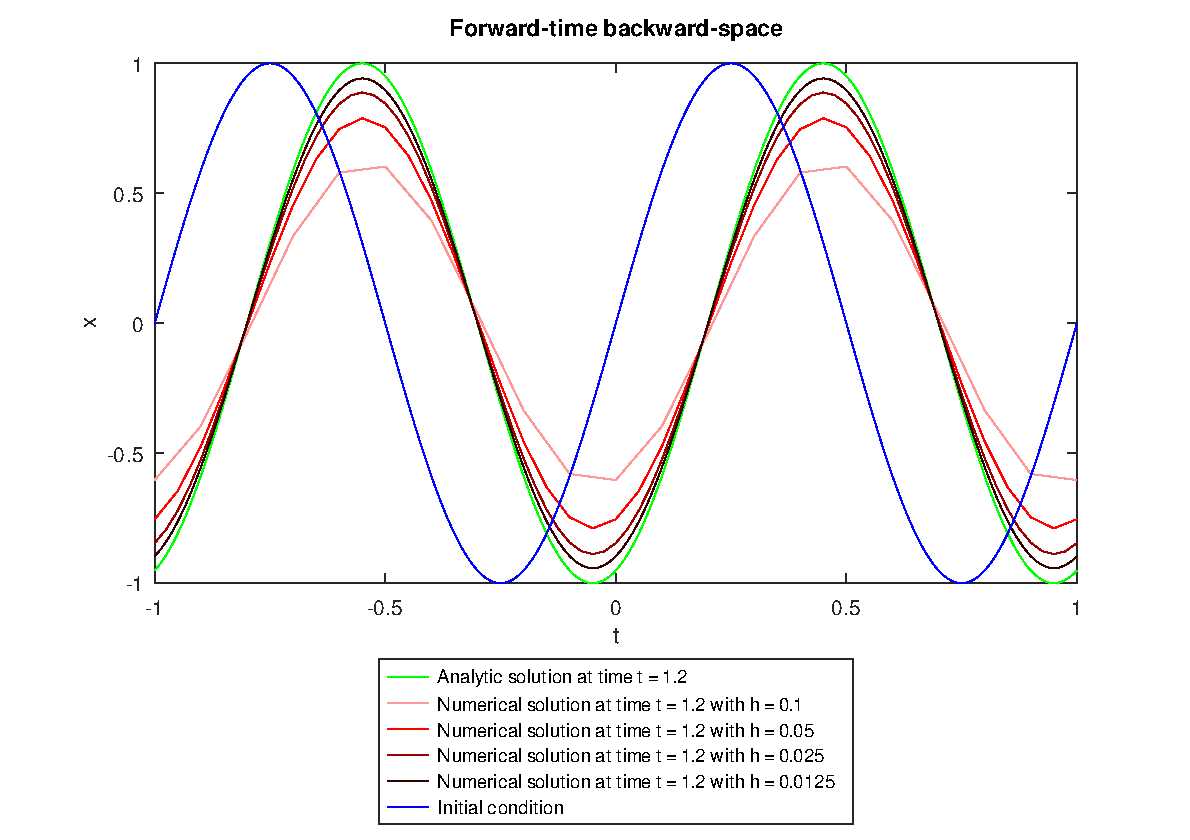
\includegraphics[width=\textwidth]{Images/ex2-ftbs.pdf}
      \caption{FTBS with $\lambda=0.8$.}
    \end{subfigure}\hfill
    \begin{subfigure}{0.49\textwidth}
      \centering
      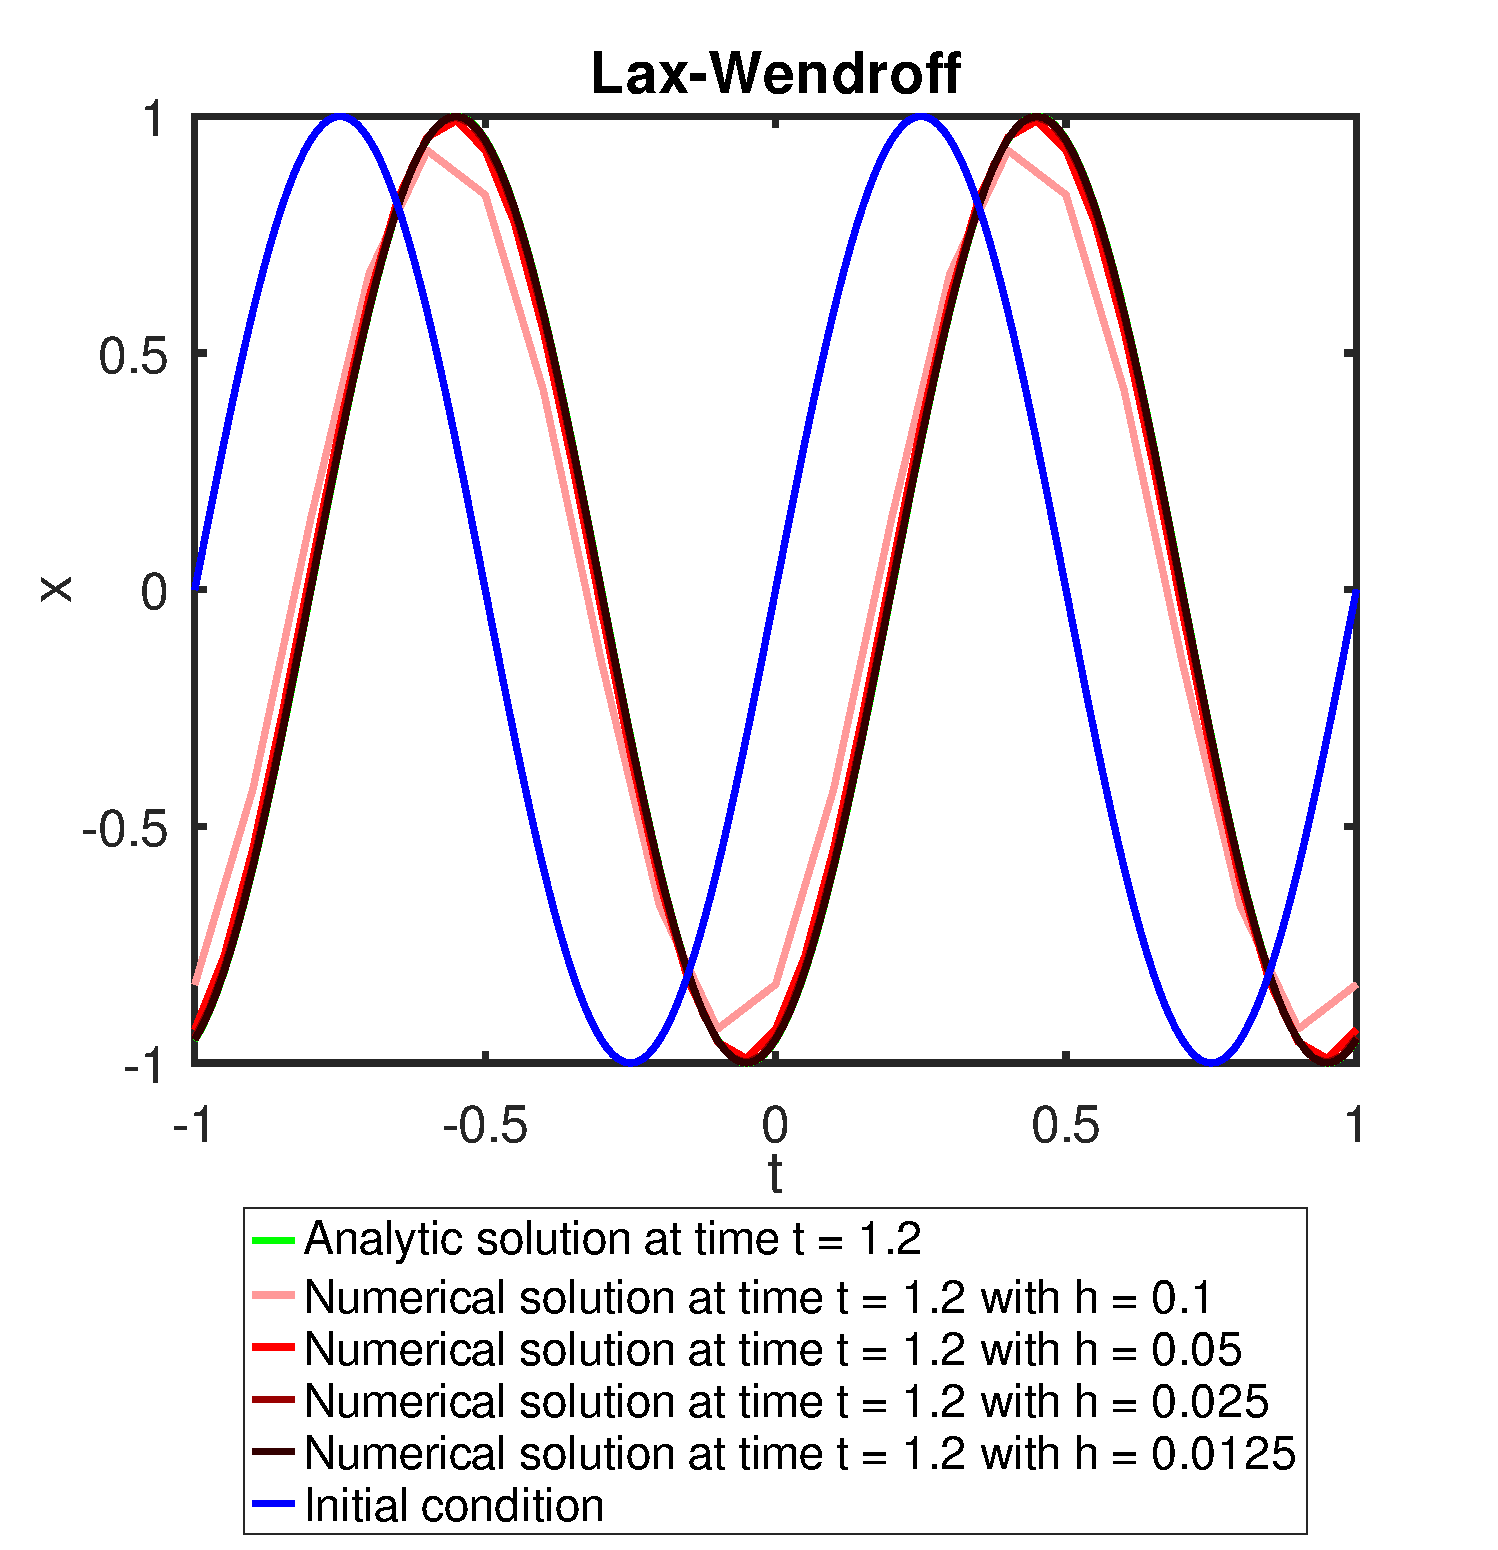
\includegraphics[width=\textwidth]{Images/ex2-lw.pdf}
      \caption{Lax-Wendroff with $\lambda=0.8$.}
    \end{subfigure}
    \caption{Plot of the analytical and numerical solutions of the convergent schemes}
  \end{figure}
\end{res}
\end{document}